
\begin{figure}[h]
    \centering
    \begin{subfigure}[b]{0.32\textwidth}
        \centering
        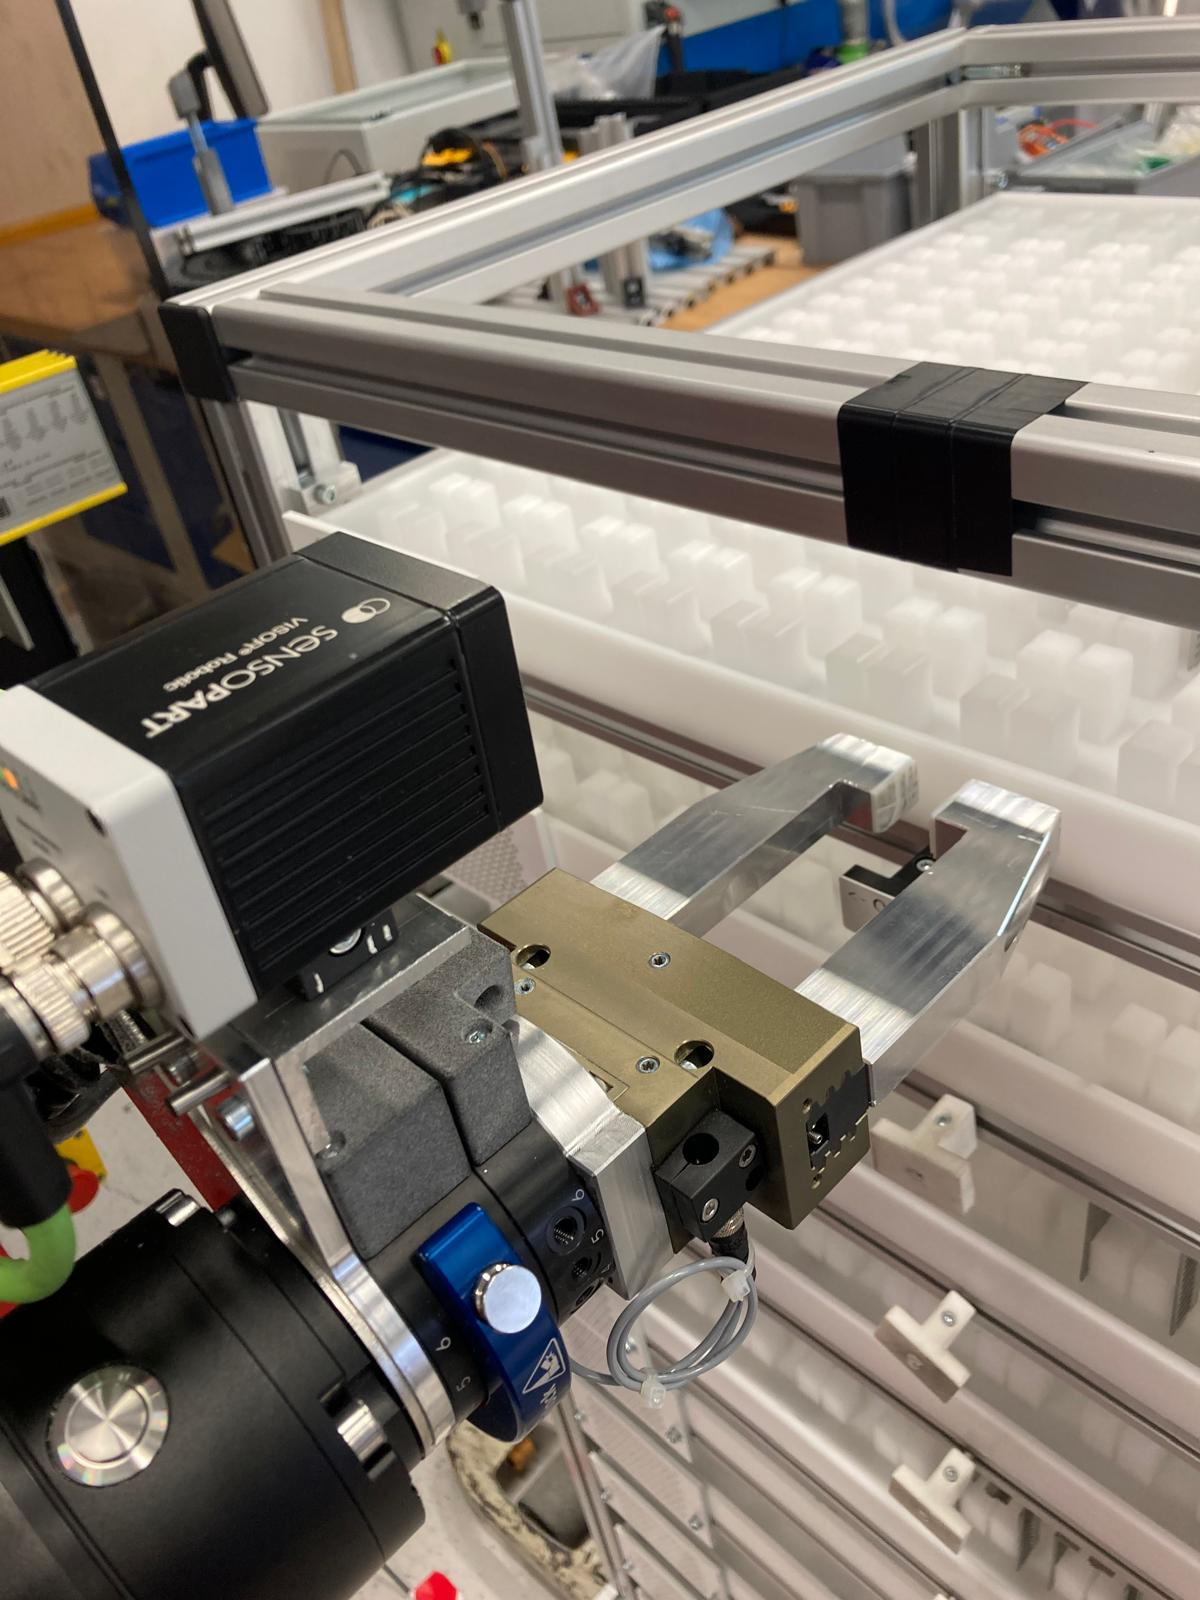
\includegraphics[width=\textwidth]{figures/shelf-control/reach-handle.jpeg}
        \caption{Reach shelf handle}
        \label{subfig:reach-handle}
    \end{subfigure}\hspace{0.1cm}
    \begin{subfigure}[b]{0.32\textwidth}
        \centering
        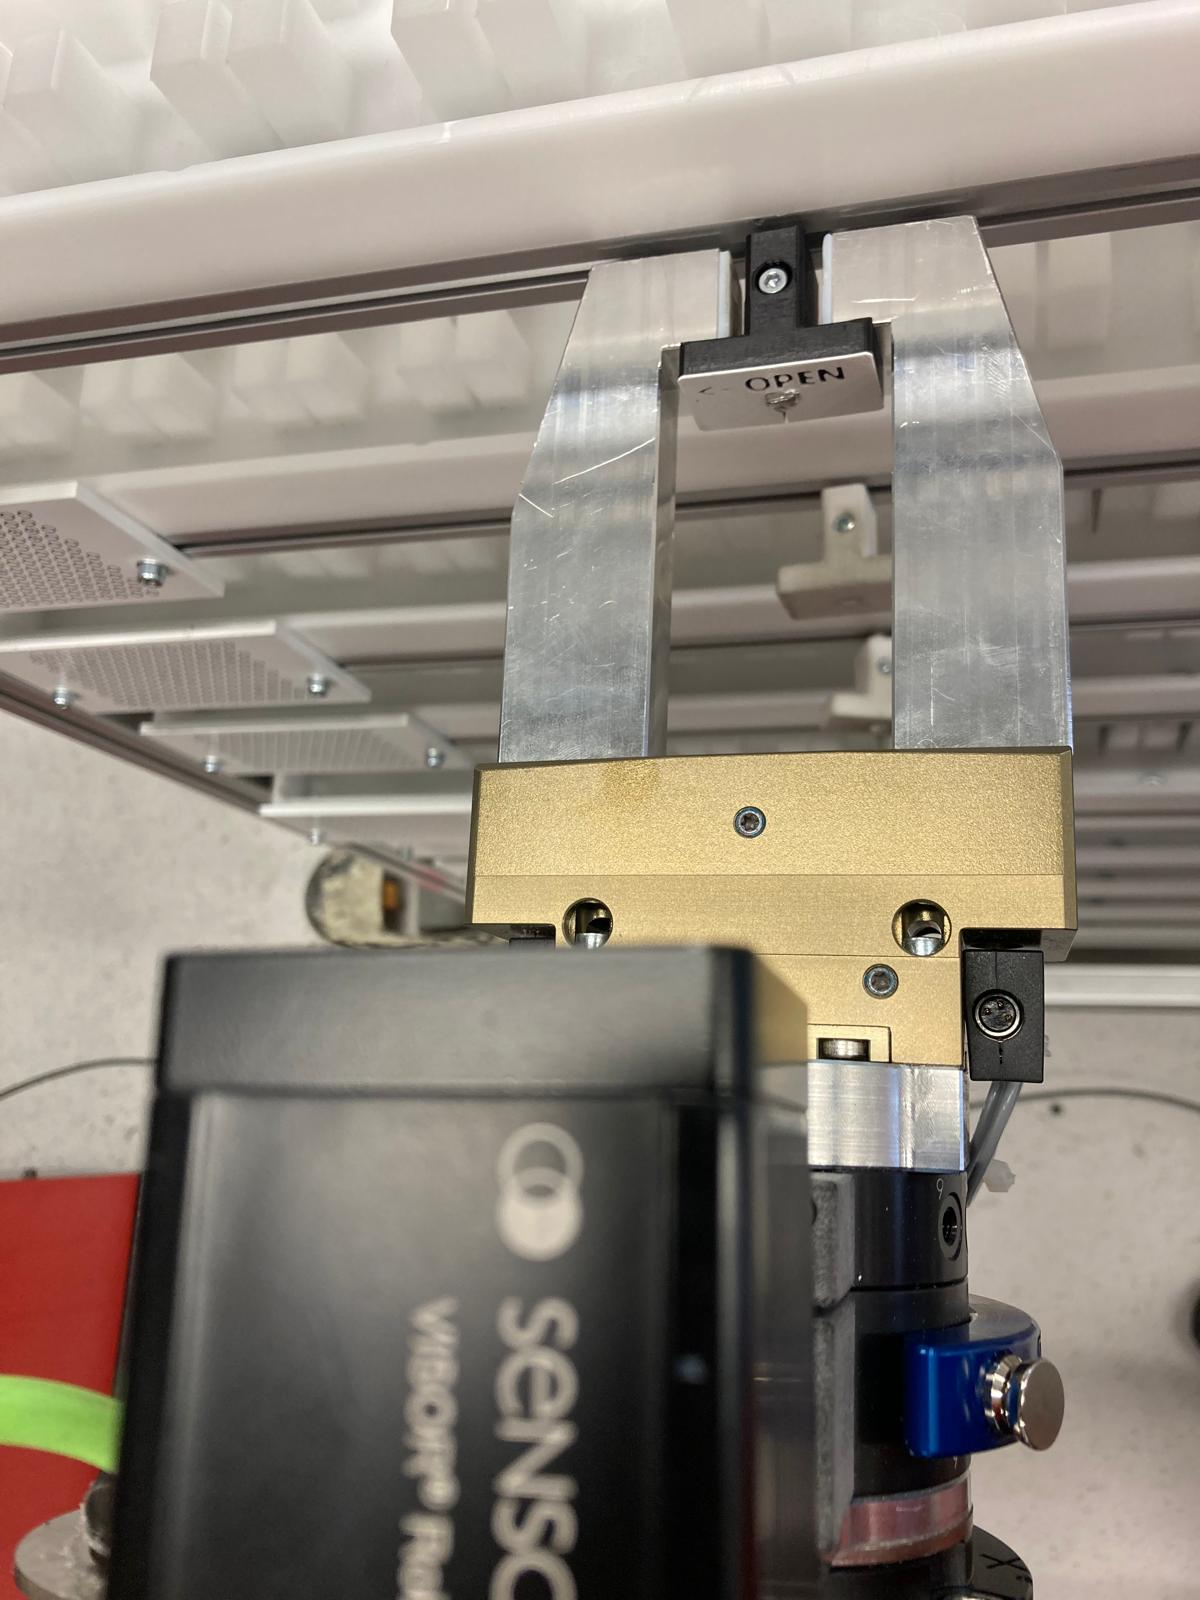
\includegraphics[width=\textwidth]{figures/shelf-control/hold-handle.jpeg}
        \caption{grasp handle with gripper}
        \label{subfig:grasp-handle}
    \end{subfigure}\hspace{0.1cm}
    \vspace{1cm}
    \begin{subfigure}[b]{0.32\textwidth}
        \centering
        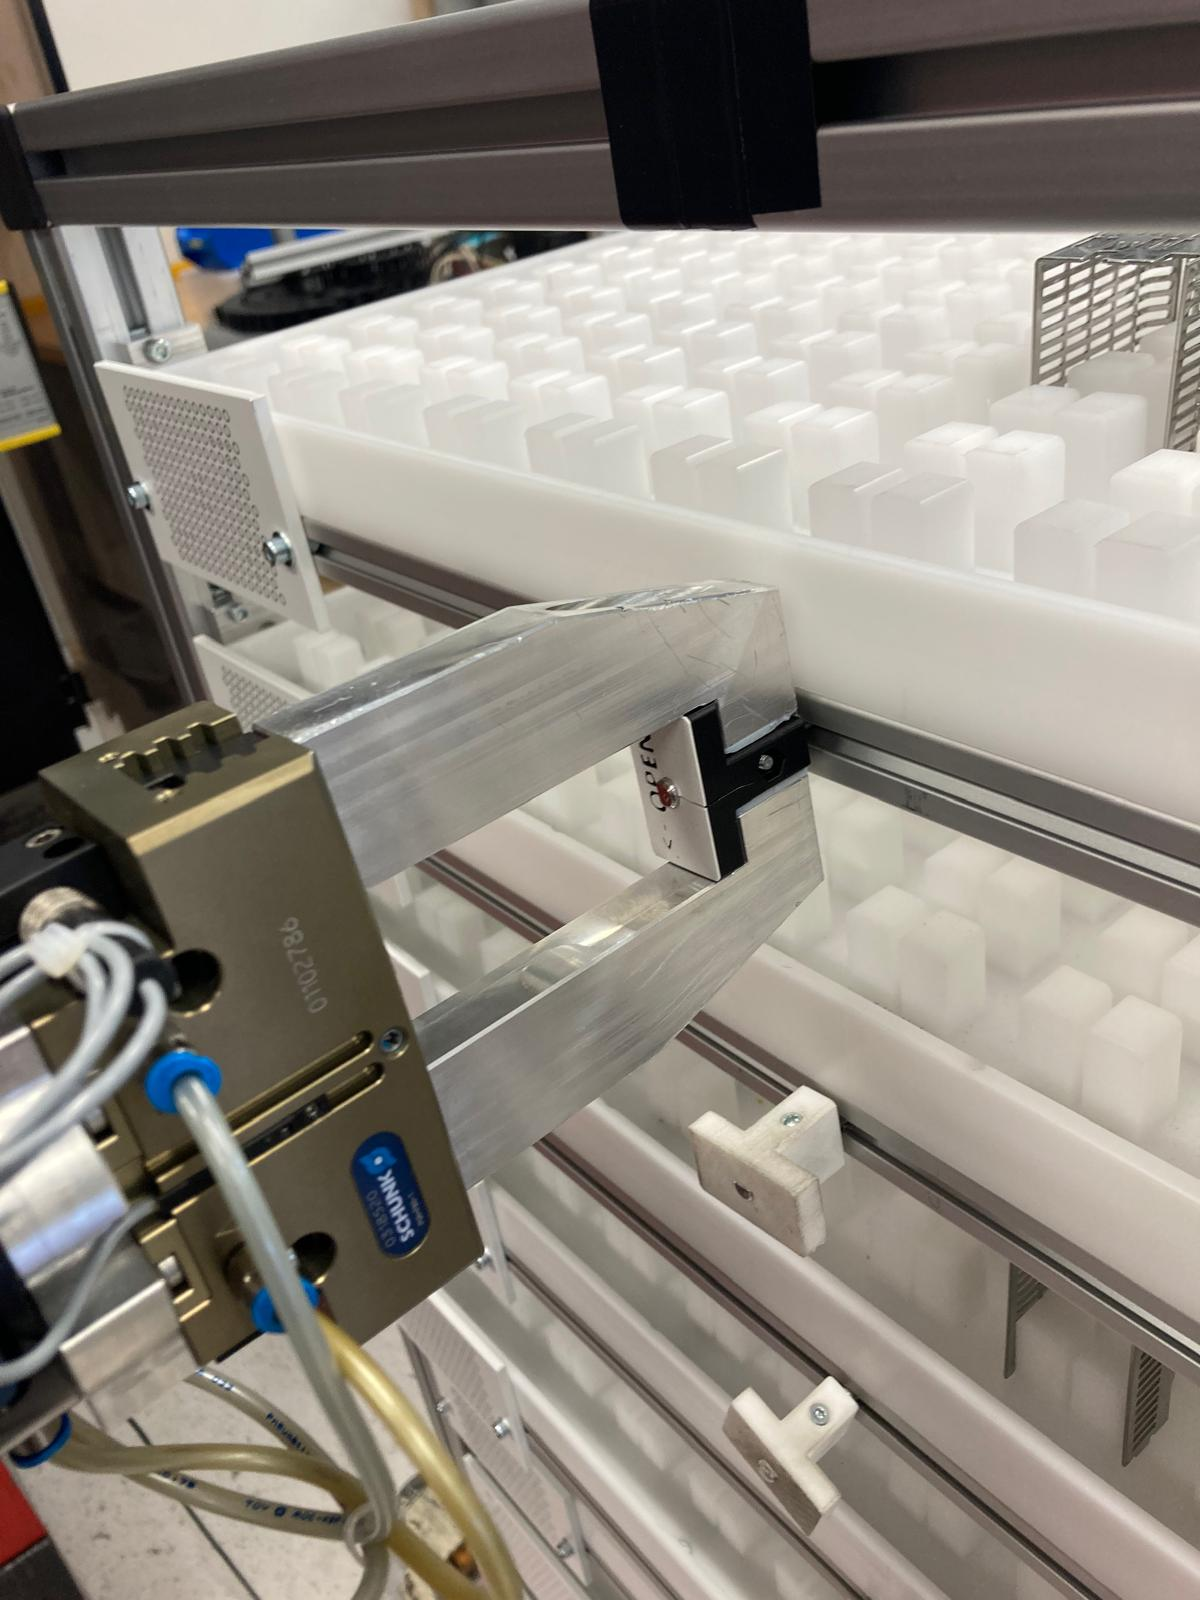
\includegraphics[width=\textwidth]{figures/shelf-control/open-handle.jpeg}
        \caption{Turn handle 100\textdegree{} to open drawer}
        \vspace{-0.45cm}
        \label{subfig:turn-open}
    \end{subfigure}\hspace{0.1cm}
    \begin{subfigure}[b]{0.32\textwidth}
        \centering
        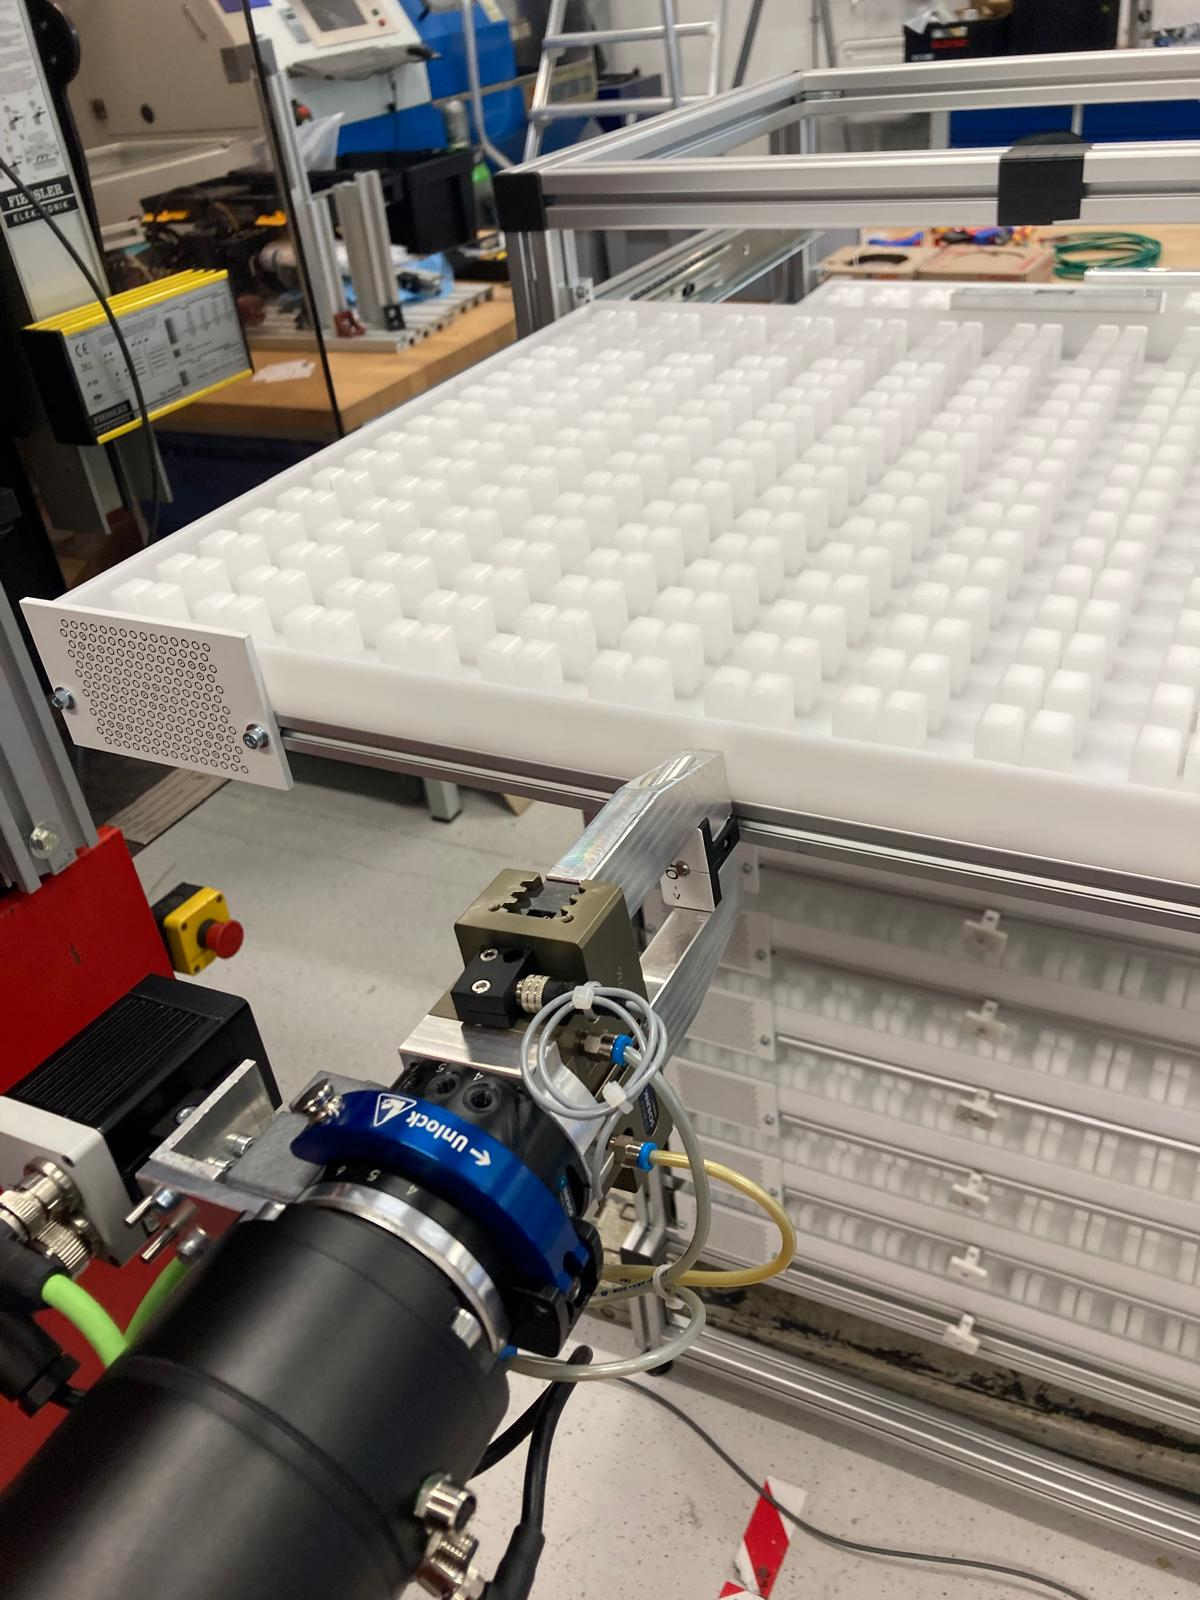
\includegraphics[width=\textwidth]{figures/shelf-control/open-drawer.jpeg}
        \caption{open drawer}
        \vspace{0.45cm}
        \label{fig:open-drawer}
    \end{subfigure}\hspace{0.1cm}
    \vspace{0.75cm}
    \begin{subfigure}[b]{0.32\textwidth}
        \centering
        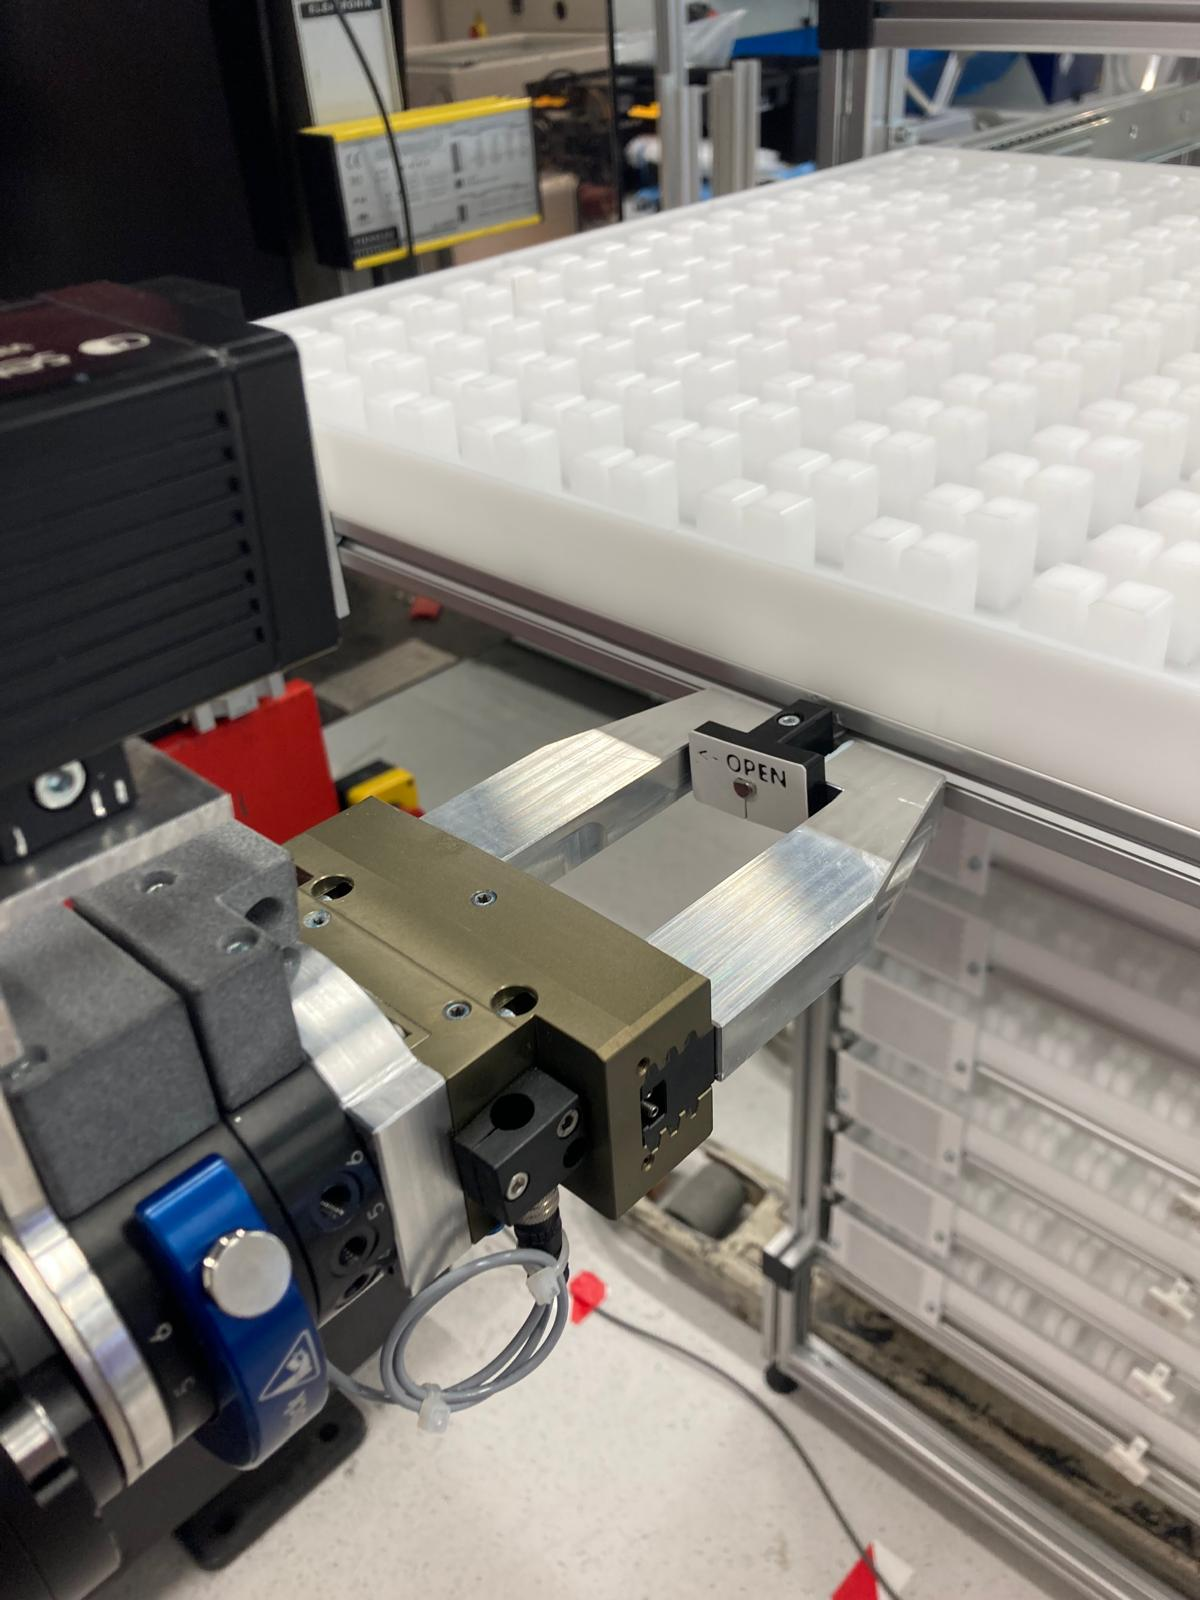
\includegraphics[width=\textwidth]{figures/shelf-control/close-handle.jpeg}
        \caption{Turn handle -100\textdegree{} to fix drawer in open position}
        \label{fig:close-handle}
    \end{subfigure}\hspace{0.1cm}
    \begin{subfigure}[b]{0.32\textwidth}
        \centering
        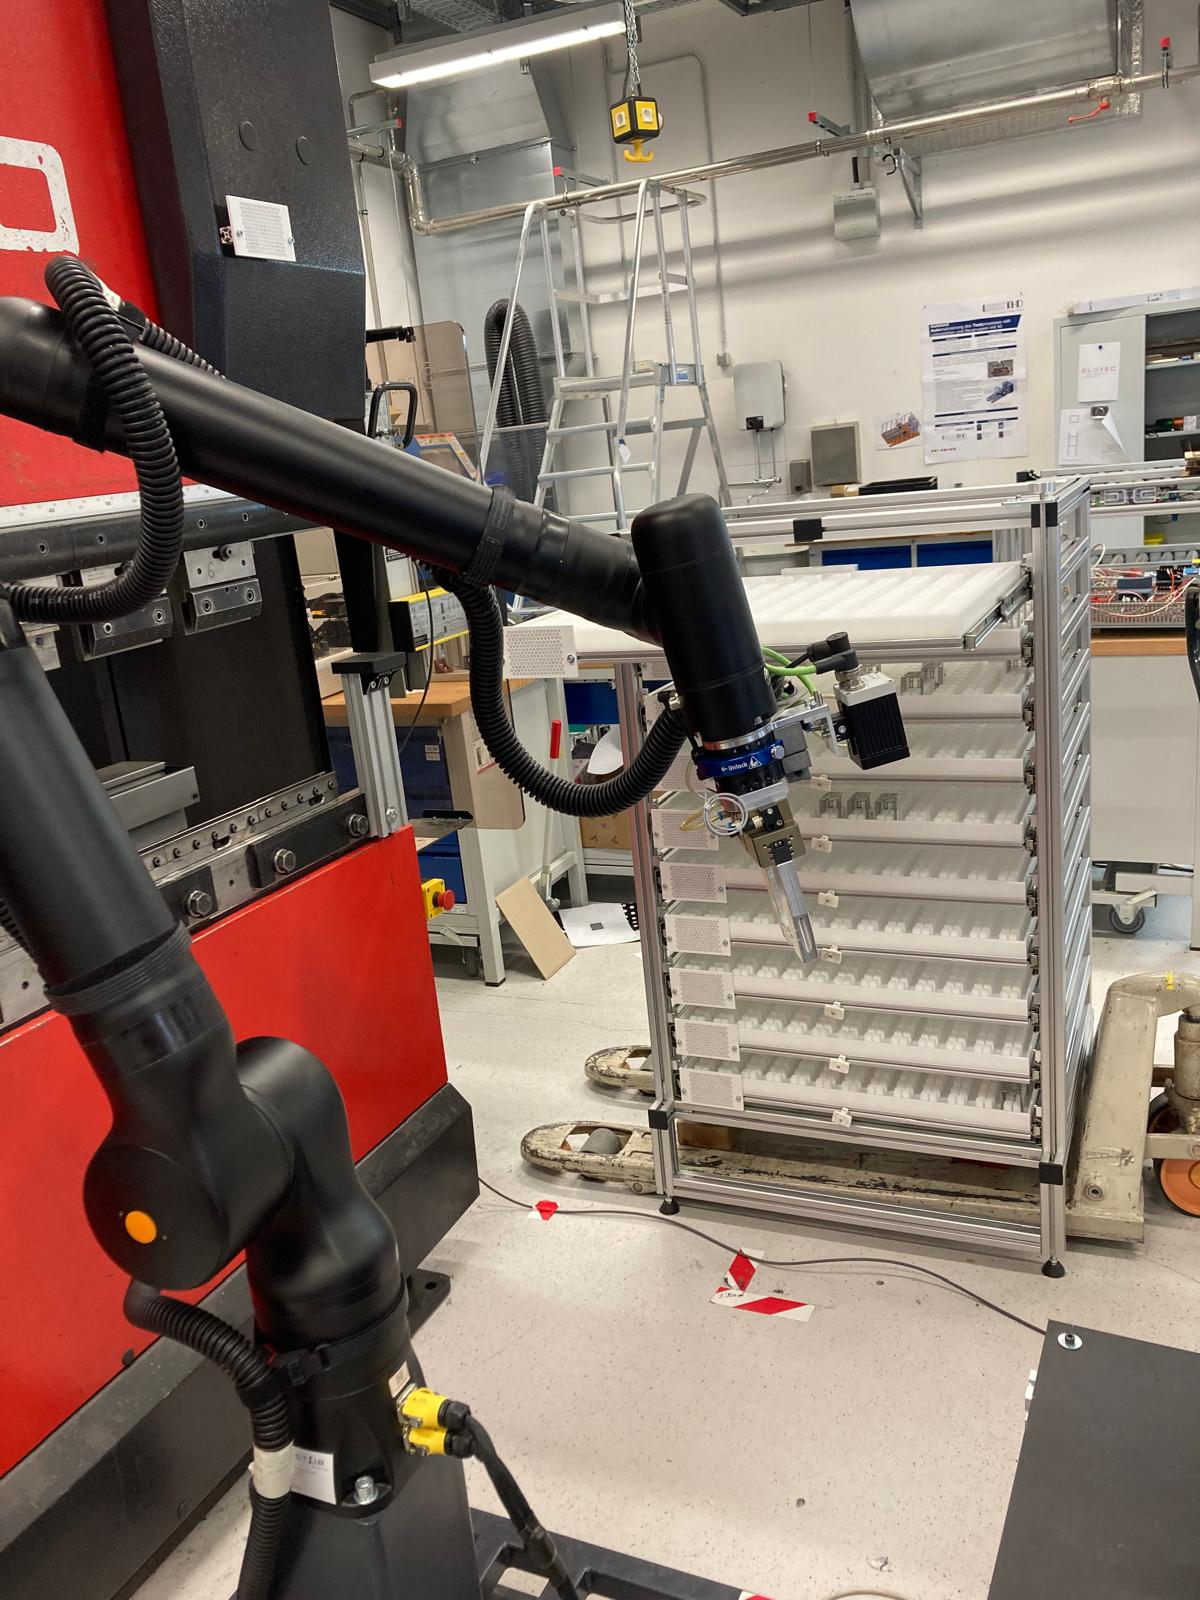
\includegraphics[width=\textwidth]{figures/shelf-control/drawer-opened.jpeg}
        \caption{Robot ready with drawer open}
        \label{subfig:drawer-opened}
    \end{subfigure}\hspace{0.1cm}
    \caption{Opening a shelf drawer for placement of bent sheet metal parts}
    \label{fig:shelf-control}
\end{figure}


